\documentclass[11pt]{article}
\renewcommand{\baselinestretch}{1.05}

\usepackage{amsmath,amsthm,verbatim,amssymb,amsfonts,amscd, graphicx}
\usepackage{graphics}

\usepackage{xcolor}

\usepackage[hidelinks]{hyperref}
\usepackage{parskip}

\usepackage{subcaption}

% Code specific

\usepackage{listings}

\definecolor{mygreen}{rgb}{0,0.6,0}
\definecolor{mygray}{rgb}{0.5,0.5,0.5}
\definecolor{mymauve}{rgb}{0.58,0,0.82}

\lstset{ %
  backgroundcolor=\color{white},   % choose the background color; you must add \usepackage{color} or \usepackage{xcolor}
  basicstyle=\footnotesize,        % the size of the fonts that are used for the code
  breakatwhitespace=false,         % sets if automatic breaks should only happen at whitespace
  breaklines=true,                 % sets automatic line breaking
  captionpos=b,                    % sets the caption-position to bottom
  commentstyle=\color{mygreen},    % comment style
  deletekeywords={...},            % if you want to delete keywords from the given language
  escapeinside={\%*}{*)},          % if you want to add LaTeX within your code
  extendedchars=true,              % lets you use non-ASCII characters; for 8-bits encodings only, does not work with UTF-8
  frame=single,	                   % adds a frame around the code
  keepspaces=true,                 % keeps spaces in text, useful for keeping indentation of code (possibly needs columns=flexible)
  keywordstyle=\color{blue},       % keyword style
  language=Octave,                 % the language of the code
  otherkeywords={*,...},           % if you want to add more keywords to the set
  numbers=left,                    % where to put the line-numbers; possible values are (none, left, right)
  numbersep=5pt,                   % how far the line-numbers are from the code
  numberstyle=\tiny\color{mygray}, % the style that is used for the line-numbers
  rulecolor=\color{black},         % if not set, the frame-color may be changed on line-breaks within not-black text (e.g. comments (green here))
  showspaces=false,                % show spaces everywhere adding particular underscores; it overrides 'showstringspaces'
  showstringspaces=false,          % underline spaces within strings only
  showtabs=false,                  % show tabs within strings adding particular underscores
  stepnumber=2,                    % the step between two line-numbers. If it's 1, each line will be numbered
  stringstyle=\color{mymauve},     % string literal style
  tabsize=2,	                   % sets default tabsize to 2 spaces
  title=\lstname                   % show the filename of files included with \lstinputlisting; also try caption instead of title
}

%

\renewcommand{\contentsname}{Table des mati\`eres}
\renewcommand\refname{R\'ef\'erences}

\topmargin0.0cm
\headheight0.0cm
\headsep0.0cm
\oddsidemargin0.0cm
\textheight23.0cm
\textwidth16.5cm
\footskip1.0cm

\begin{document}

\title{\textbf{Projet de Conception en Micro\'electronique Analogique} \\ R\'ealisation d'un CAN FLASH 6 bits}
\author{Ferdinand Goumis \\ Mohamed Hage Hassan \medskip\\\medskip \textbf{Encadrants} \medskip \\ Fatah Ellah Rarbi \\ Daniel Dzahini \\ Florent Cilici \\ Laurent Aubard}
\date{24 Avril 2017}
\maketitle
\thispagestyle{empty}

\renewcommand{\abstractname}{Abstrait(Pr\'emabule)}

\begin{abstract}
Quisque hendrerit finibus lacus pulvinar semper.
Donec rutrum lacinia tempus. Aenean ligula sapien, euismod vel arcu sit amet,
molestie sollicitudin nisl. Pellentesque habitant morbi tristique senectus et netus et
malesuada fames ac turpis egestas. Nullam ac ornare ante, efficitur rhoncus justo.
Sed tristique lobortis nisl a gravida. Etiam id purus ut enim sagittis auctor id ac quam.
Fusce vulputate nisi rutrum, aliquam neque et, auctor risus. Quisque commodo molestie felis,
sed egestas sem. Sed euismod, turpis id dignissim malesuada, elit nulla auctor elit, nec hendrerit
ipsum odio quis ex. Sed sollicitudin fringilla purus, et dignissim risus auctor eget. Etiam bibendum,
nisi at posuere mattis, dui risus hendrerit sapien, vitae feugiat libero magna sollicitudin leo.

\begin{center}
  \textbf{\textcolor{red}{\'Elimine le lorem Ipsum apr\`es.}}
\end{center}

\end{abstract}

\vskip 7cm
\begin{center} \textbf{Institut Polytechnique de Grenoble} \end{center}

\clearpage

\tableofcontents
\clearpage

\section{Introduction}

Lorem ipsum dolor sit amet, consectetur adipiscing elit. Morbi tincidunt ut risus eget feugiat.
Etiam eget viverra purus, sed iaculis dui. Duis vel urna tempus, placerat dolor ut, molestie erat.
Praesent non dapibus tortor. Vestibulum facilisis mollis urna a fringilla. Nulla consequat lacus in dolor mattis varius.
Praesent pharetra, mauris quis pretium tincidunt, tortor risus lobortis leo, sit amet mattis metus leo a dolor.
 Curabitur mi risus, lacinia a lacus ut, porta hendrerit quam. Ut dignissim fermentum bibendum.
 Mauris auctor tincidunt enim, nec auctor mi faucibus quis. Sed volutpat augue non ligula iaculis, pharetra elementum dolor accumsan.
 Duis semper semper erat id accumsan. Cras consectetur varius varius. Sed porta semper tellus, quis auctor lacus euismod cursus.

\textit{Note :} Certaines illustrations sont extraites des projets.

\section{Cahier des charges}
Le projet n\'ecessite d'avoir :
\begin{itemize}
\item[-] Une r\'esolution du CAN-FLASH de 6 bits, ce qui implique l'utilisation de $2^{6} -1 = 63 $ comparateurs.
\item[-] Dynamique du signal en entr\'ee $V_e \in [0.5 V,\phantom{2} 2.5V]$
\item[-] Fr\'equence d'\'echantillonnage : $f_h = 20 MHz $
\item[-] \textbf{\textcolor{red}{Plus..}}
\end{itemize}

\section{M\'ethodologie de travail}
Notre m\'ethode de travail tout au long du projet consiste \`a :
\begin{itemize}
  \item[-] D\'ecoupage du CAN-FLASH en \'el\'ements fonctionnels.
  \item[-] Compr\'ehension du fonctionnement du bloc.
  \item[-] Mise en place d'un sch\'ema en \'el\'ements ideaux et v\'erfication du fonctionnement attendu par simulations.
  \item[-] \'Etude th\'eorique pour le bloc r\'eel, dimensionnement des transistors et mise en validation par reproduction
  d'un sch\'ema et simulations.
  \item[-] Mise en place d'un sch\'ema global pour sa validation en simulation (Echantillonneur-Bloqueur par example).
\end{itemize}

\clearpage

\section{Mise en place de l'\'echantillonneur-bloqueur}
Pour qu'on puisse convertir le signal, on doit impl\'ementer une \'etape d'\'echantillonnage, avec un fonctionnement \`a haute fr\'equence,
 avant la r\'ealisation de l'\'etape de comparaison, qui consiste \`a comparer les diff\'erents niveaux obtenus par \'echantillonnage avec l'amplitude du signal initial,
  modifi\'ee par le pont de diviseurs de tensions.

On utilise alors une topologie d'un \'echantilloneur-bloqueur \`a capacit\'es commut\'ees:

\begin{figure}[!htb]
\begin{center}
  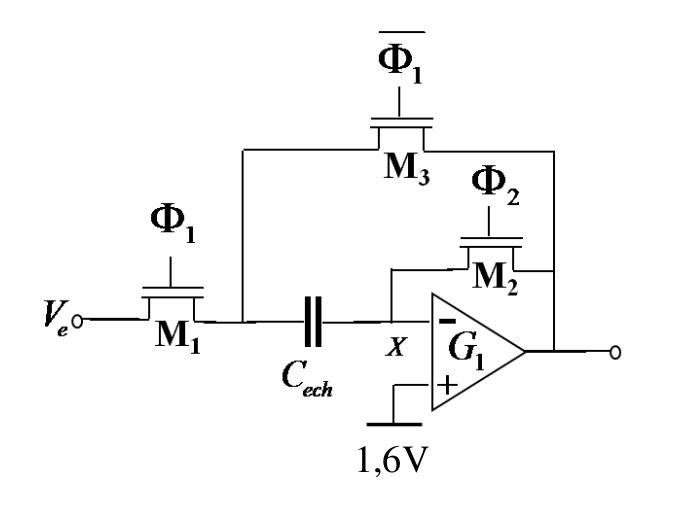
\includegraphics[scale=0.30]{Echantillonneur-bloqueur.jpg}
  \caption{Sch\'ema d'un \'echantilloneur-bloqueur \`a capacit\'es commut\'ees}
\end{center}
\end{figure}

\subsection{Principe de fonctionnement}

\begin{center}
    \textbf{Explication des diff\'erents phases de fonctionnement + \textcolor{red}{d\'emonstrations th\'eoriques}}
\end{center}

\clearpage

\subsection{Simulation avec des \'el\'ements id\'eaux}

\begin{figure}[!htb]
\begin{center}
  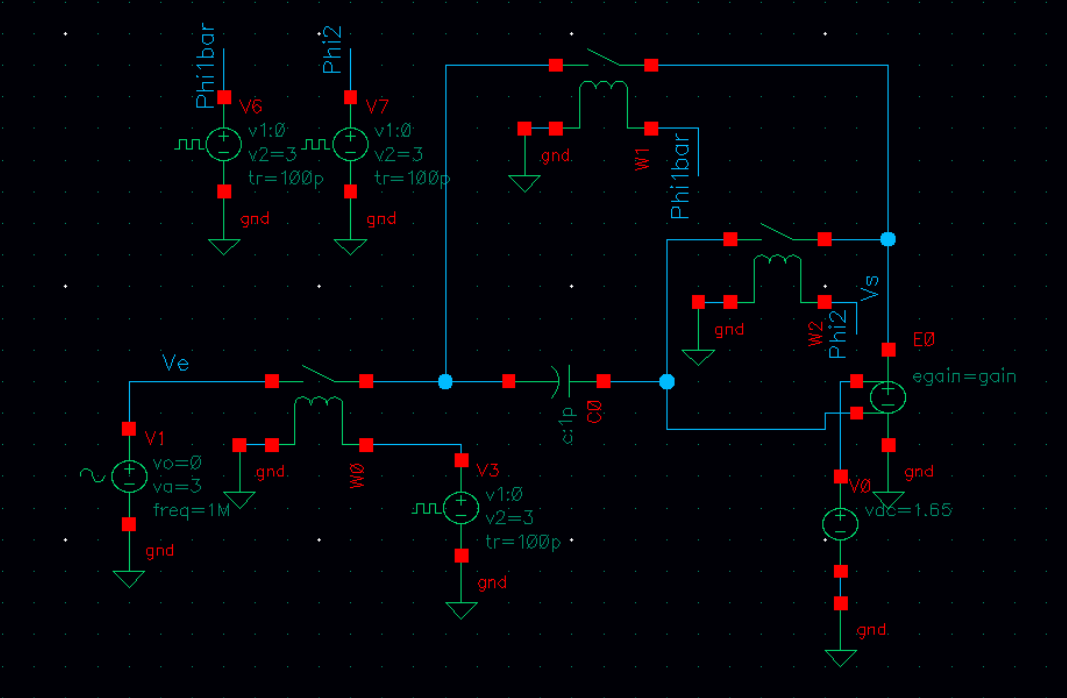
\includegraphics[scale=0.35]{Echantillonneur-bloqueur_ideal.png}
  \caption{Sch\'ema de l'\'echantilloneur-bloqueur en \'el\'ements ideaux}
\end{center}
\end{figure}

\clearpage

\subsection{R\'ealistation des switchs r\'eels et simulations}

\textbf{Vue th\'eorique et Dimmensionnements}

\begin{figure}[!htb]
\begin{center}
  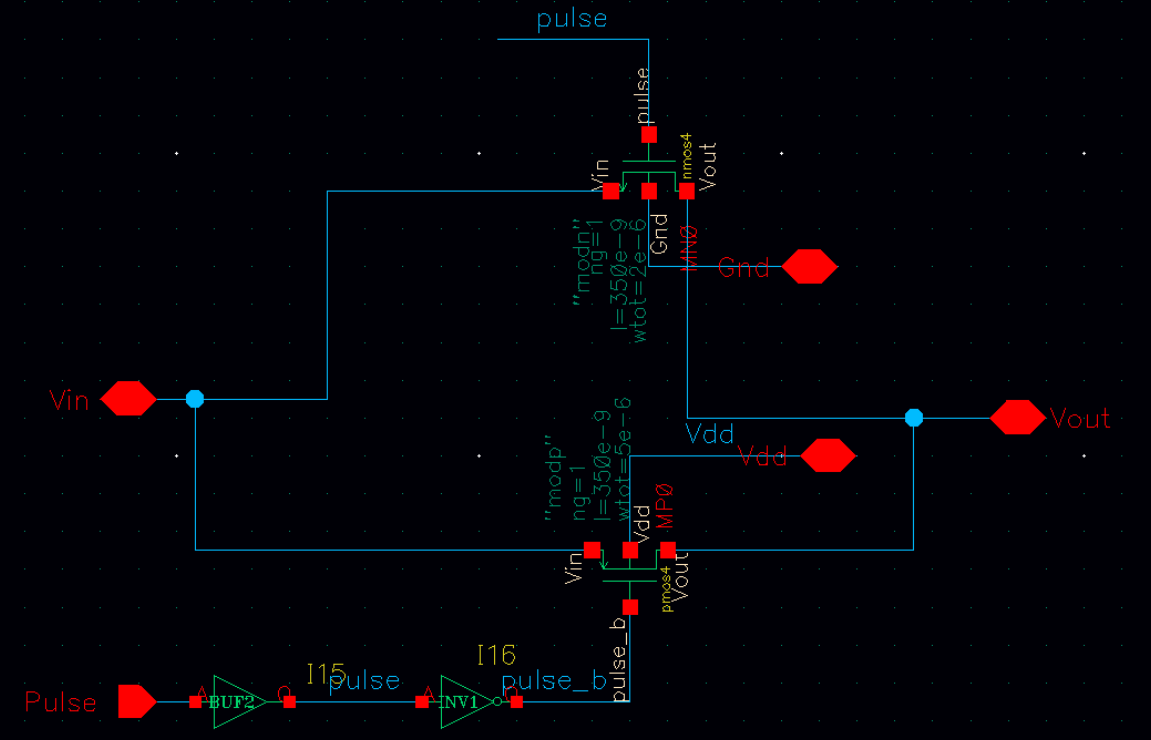
\includegraphics[width=0.8\linewidth]{switchs_.png}
  \caption{Sch\'ema \'electrique des switch en CMOS}
\end{center}
\end{figure}

\textbf{V\'erification des performances par simulations}

\begin{figure}[!htb]
\begin{center}
  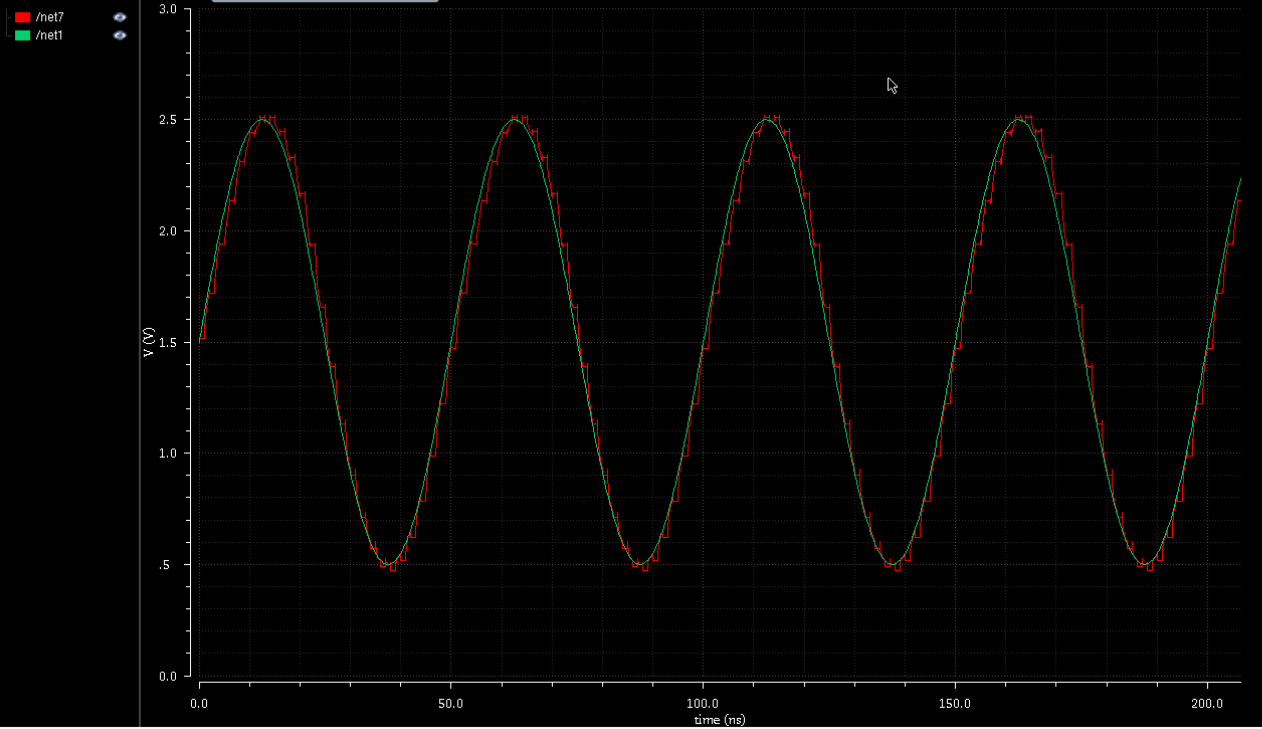
\includegraphics[width=0.8\linewidth]{switchs_simu.png}
  \caption{Sch\'ema \'electrique des switch en CMOS}
\end{center}
\end{figure}



\clearpage

\subsection{Simulation finale}
En rassemblant tous les \'el\'ements, on aboutit au sch\'ema suivant :

\begin{figure}[!htb]
\begin{center}
  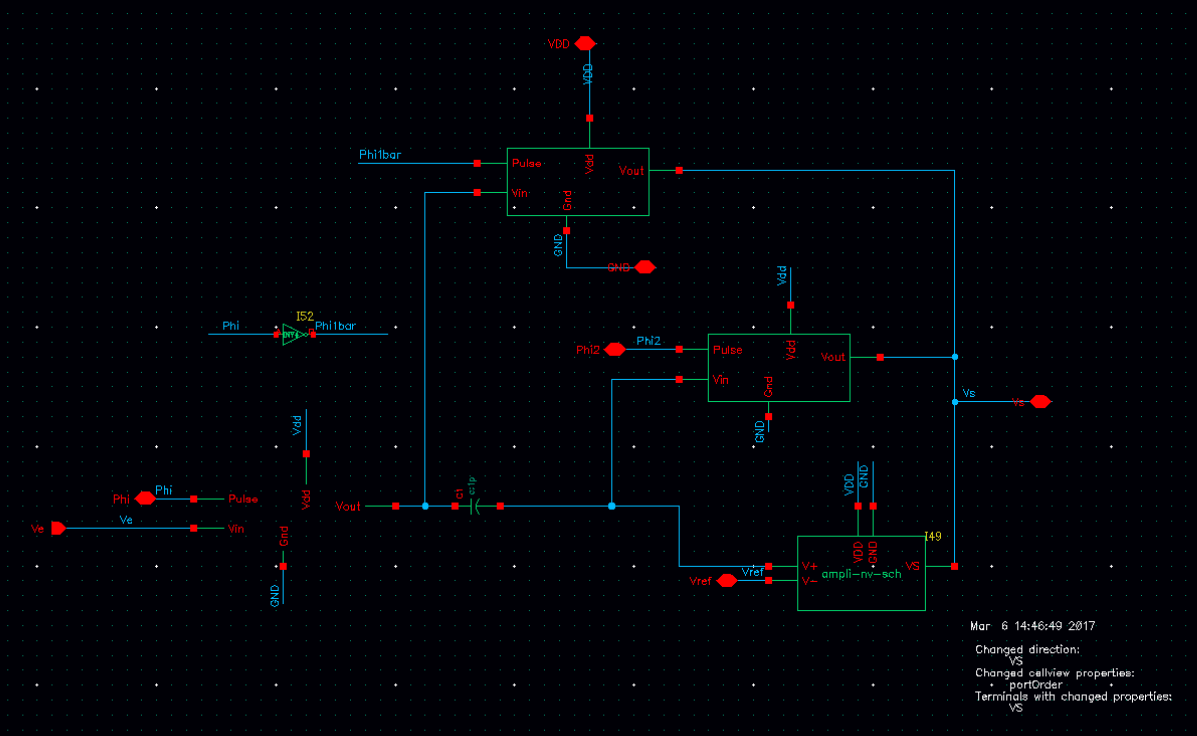
\includegraphics[width=0.8\linewidth]{EB-Schematic.png}
  \caption{Sch\'ema de l'\'echantilloneur-bloqueur r\'eel}
\end{center}
\end{figure}

Effectuant la simulation :

\begin{figure}[!htb]
\begin{center}
  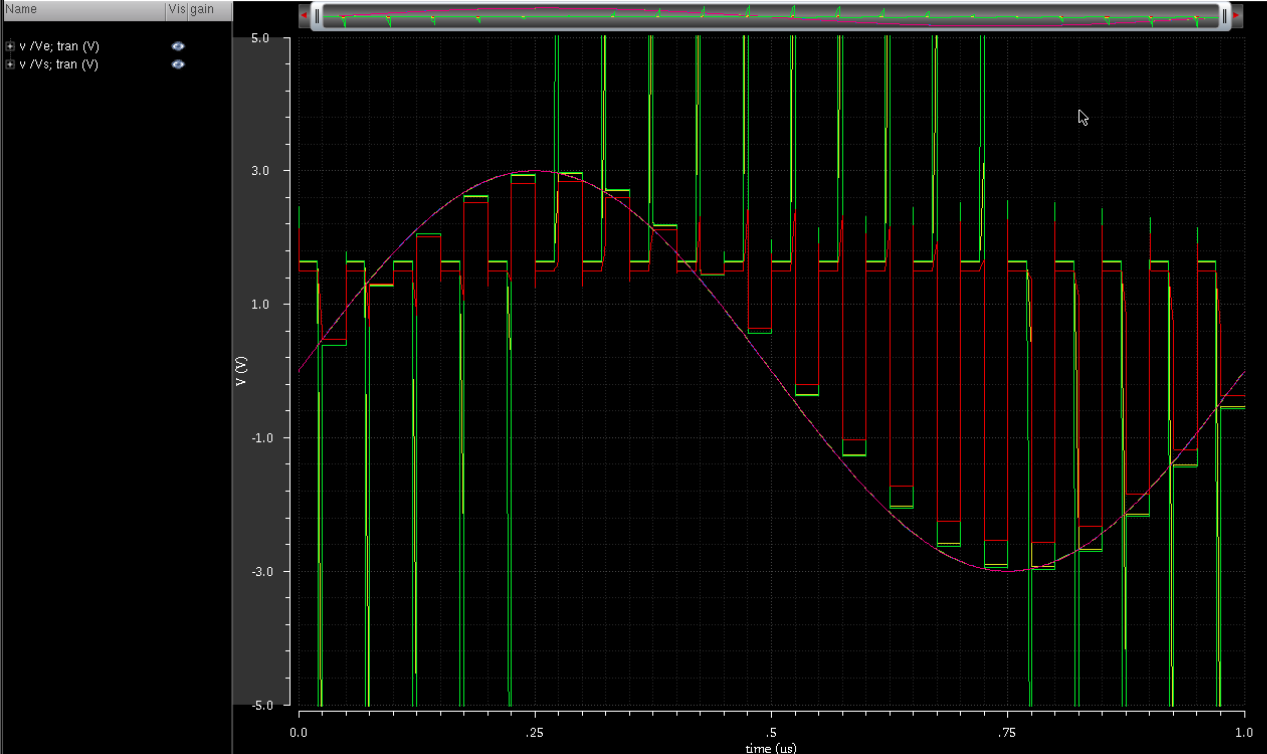
\includegraphics[width=0.8\linewidth]{simu_ech_bloqueur.png}
  \caption{Sch\'ema de l'\'echantilloneur-bloqueur r\'eel}
\end{center}
\end{figure}


\clearpage
\section{R\'ealisation d'un Amplificateur OTA \`a deux \'etages}

\subsection{Cahier des charges}

\textbf{Le cahier de charges n\'ecessite :}
\begin{itemize} \itemsep -2pt
  \item[-]
  \item[-]
\end{itemize}

\subsection{Calcul th\'eorique et dimensionnements}

\begin{figure}[!htb]
\begin{center}
  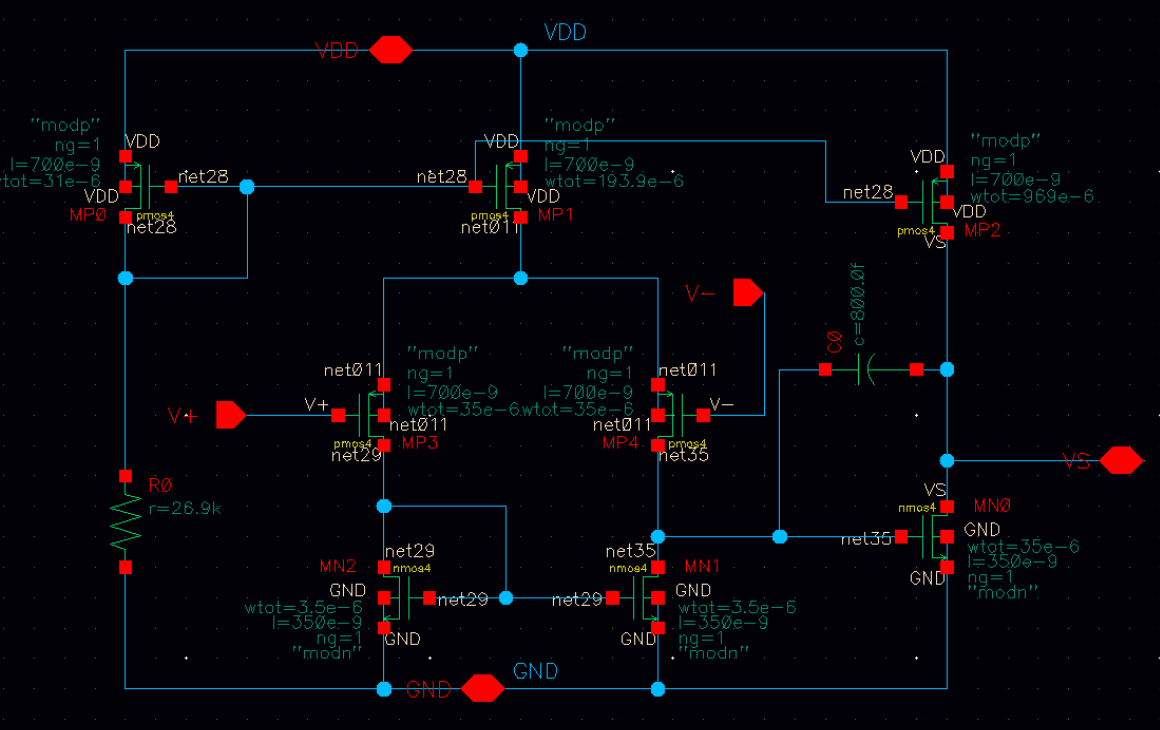
\includegraphics[width=\linewidth]{amplificateur_.png}
  \caption{Architecture de l'amplificateur \`a deux \'etages apr\`es dimensionnements}
\end{center}
\end{figure}

\clearpage

\subsection{Simulation et optimisation}

\begin{figure}[!htb]
\begin{center}
  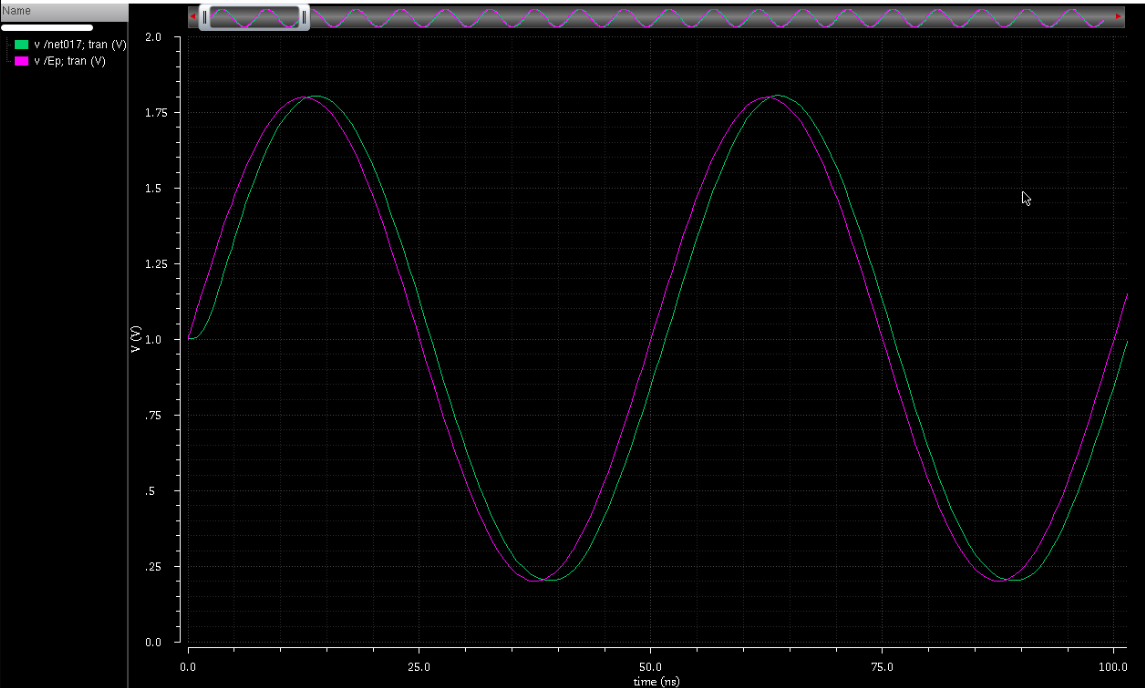
\includegraphics[width=\linewidth]{reponse_ampli.png}
  \caption{Architecture de l'amplificateur \`a deux \'etages apr\`es dimensionnements}
\end{center}
\end{figure}


\clearpage

\section{Mise en oeuvre des comparateurs synchronis\'es par horloge}
\subsection{Principe de fonctionnement}
L'\'etape suivante est la cr\'eation de 63 comparateurs et seuils afin d'au mieux \'evaluer le niveau de
notre signal \`a chaque front sur un cycle d'horloge commune \`a tous les blocs.

\begin{figure}[!htb]
\begin{center}
  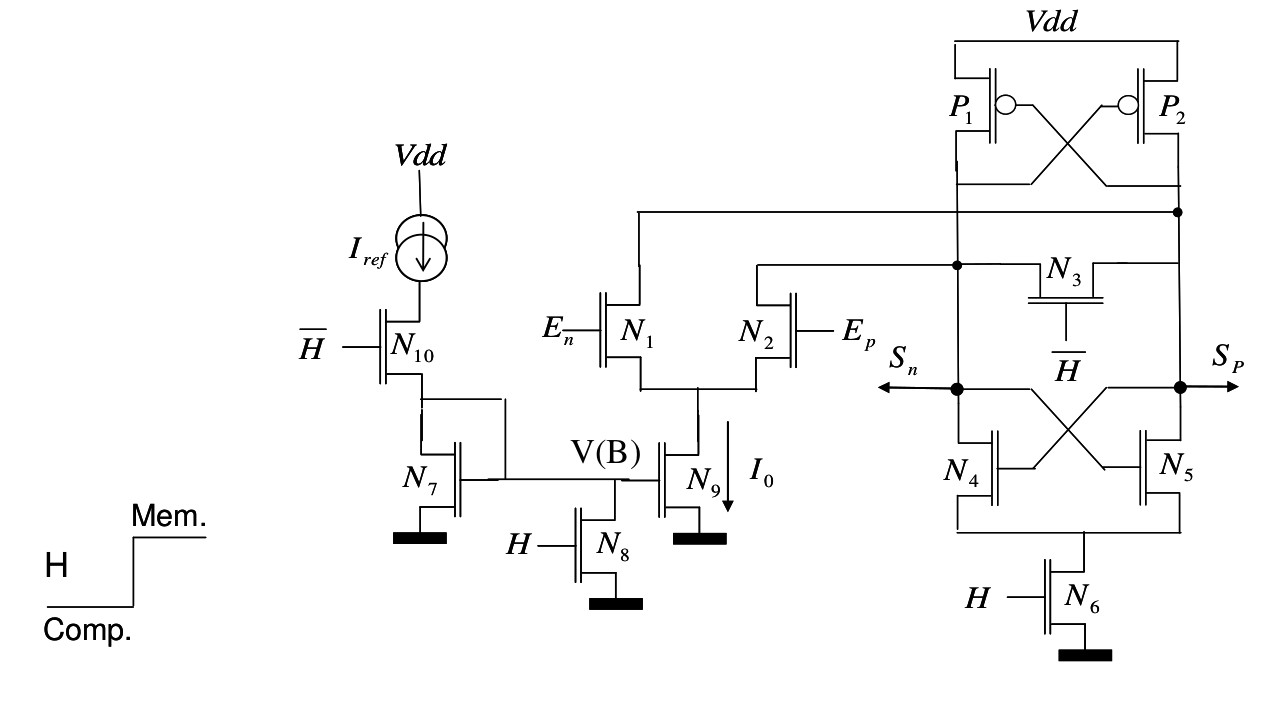
\includegraphics[scale=0.38]{comparateur_schema.jpg}
  \caption{Architecture des comparateurs synchronis\'es par horloge avec une paire crois\'ee}
\end{center}
\end{figure}

La structure utilis\'ee pour ce comparateur et bri\`evement d\'ecrite dans le sujet, et illustr\'ee par
la figure X, utilise un courant provenant d'un miroir de courant (partie gauche de la structure).
La propri\'et\'e comparatrice est effectu\'ee par la paire diff\'erentielle $N_1$/$N_2$ Ensuite, la partie de droite
($P_1$,$P_2$ et $N_3$,$N_4$,$N_5$,$N_6$) fait basculer le comparateur soit en satur\'e (sortie de 3.3 V)
ou \`a la masse \`a travers le transistor $N_6$ qui est alors passant.

\subsection{Partie Th\'eorique}
Afin d'au mieux dimensionner ce comparateur, nous avons effectu\'e les hypoth\`eses et calculs suivants,
par rapport au courant et aux dimensions des transistors:

\subsubsection{Phase de comparaison (niveau d'horloge bas)}

Pour $V_{EP}-V_{EN}$ tr\`es diff\'erent de $0$ (cas d'une entr\'ee repr\'esentant le signal et l'autre un seuil),
le courant $I_0$ capable de charger ou d\'echarger la capacit\'e aux nœuds $S_N$ ou $S_P$ en $\frac{1}{4}$ de
p\'eriode d'horloge sur une variation de $V_{DD}$ vaut :

\[
I_0 = C \frac{V_{DD}}{t} = 26 \mu A
\]

si l'on consid\`ere un temps de 12.5 ns = $\frac{1}{4} \times T_{horloge}$ \`a 20 MHz.

A l'\'equilibre ($V_{EN} = V_{EP}$), pour avoir une tension de mode commun en sortie
$V_{SN} = V_{SP} = \frac{V_{DD}}{2}$ , le rapport $\frac{W}{L}$ de $P_{1,2}$ vaut :

\[
  \bigg(\frac{W}{L}\bigg)_{P1,2} = \frac{I_D}{K_P (V_{dd}/2 - |V_{TP}|)^{2}} = 1.229
\]

Afin que les transistors $N_{1,2}$ pr\'esentent une capacit\'e $C_{GS}$ en entr\'ee compatible
ou inf\'erieure \`a celle prise en compte pour fixer $C_s$ dans le calcul de l'\'echantillonneur
bloqueur, la relation :

\[
  C_{GS} = \frac{2}{3} C_{ox} W_{N_{1,2}} L \leq C_{comp}
\]

Ce qui implique que $W_{N_{1,2}} \leq 68 \mu m$ puisque :

\[
  C_S = C_{ech} + 63 \times C_{comp}
\]
et que :
\[
  C_{comp} = \frac{5}{63} \phantom{2} pF = 79 fF
\]

D\'eterminons maintenant les tailles des transistors servant \`a polariser la paire N1/N2 :

Si l'on remplace $N_{9}$ par un g\'en\'erateur de courant de valeur $I_{0}$, une simulation DC
sous Cadence donne une valeur de tension au noeud A : $V_A = 0.75 V$.

Afin que la grille du transistor $N_9$ soit polaris\'e avec la condition $V_{GS}-V_{tn}=V_{DS} - 0,2V$
 (0,2V au-dessus de la limite de zone active), nous en d\'eduisons la tension au noeud B : $V_B = 1.12 V$

Puis, le calcul de $\frac{W}{L}$ de $N_9$ vient avec :
\[
  I_d = K_n \frac{W}{L} (V_{gs} - V_{tn})^2 \bigg( 1 + \frac{K_{en}}{L} V_{ds}\bigg)
\]

Le transistor est au-dessus de la LZA :

\[
\bigg(\frac{W}{L} \bigg)_{N_9} = \frac {26µA}{55µA . (V_B - V_T)^2 ( 1+ (0.03/0.35) V_A)}
\]
\[
\bigg(\frac{W}{L} \bigg)_{N_9} = 1.46
\]

Nous faisons de m\^eme afin de calculer les dimensions du transistor $N_7$ avec la condition
$I_{ref} =\frac{I_0}{2}$

Pour calculer celui de N7, m\^eme formule sauf que :
\[
  \bigg(\frac{W}{L} \bigg)_{N_7} = \frac {\frac{26}{2}µA  }{55µA . (V_B - V_T)^2 ( 1+ (0.03/0.35) V_B)}
\]
\[
\bigg(\frac{W}{L} \bigg)_{N_7} = 0.72
\]

On prendra pour $N_{10}$ un $W = 5 \mu m$.

Le calcul des dimensions du transistor $N_8$ s'effectue en consid\'erant qu'il peut charger ou d\'echarger
la capacit\'e estim\'ee par simulation au noeud B en $\frac{1}{4}$ de p\'eriode d'horloge.

\[
I_{N_8} = \frac {V_B C_B}{\frac{1}{4} T_H} = 2 µA
\]

\iffalse
\textbf{\textcolor{red}{Mettre les simulations}}
\fi

\subsubsection{Phase de m\'emorisation (niveau d'horloge haut)}

Afin que la chute de tension dans le transistor $N_6$  \`a l'\'etat ON soit de l'ordre de $0,5 V$ lorsque $H=1$
pour un courant $I_{N_6}= I_0$, il vient :
\[
  \bigg(\frac{W}{L} \bigg)_{N_6} = 0.19
\]

car la chute de tension \`a travers la r\'esistance ON du transistor vaut $R_{ON} \times I_0 = 0.5V$

Pour une tension de mode commun en sortie $V_{SP}=V_{SN} = \frac{V_{dd}}{2}$,

\[
  \frac{I_0}{2} = K_n \frac{W}{L}(1.65-0.5 - V_{tn})^2
\]
\[
  \bigg(\frac{W}{L} \bigg)_{N_{4,5}} = 0.70
\]

\clearpage

\begin{figure}[!htb]
      \centering
      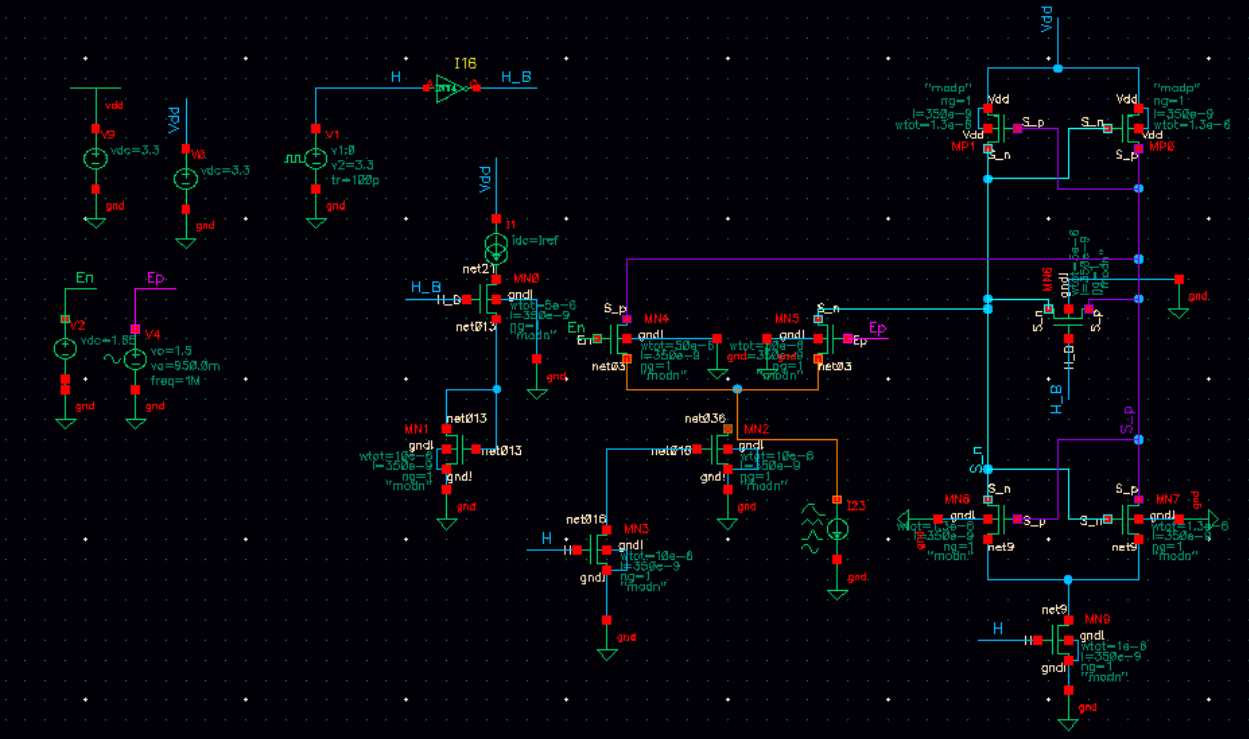
\includegraphics[width=0.9\linewidth]{comparateur_schema_cadence_.png}
      \caption{Sch\'ema \'electrique}
      \label{fig:schcomp}
\end{figure}%


\subsection{Simulations/Optimisations}

Finalement, les simulations pr\'esentent un comparateur qui est approximatif : la sortie en mode
commun n'est jamais r\'eellement soit \`a 0 ou \`a 3.3 V. En effet, le z\'ero logique se situe autour de 1.65 V
et le 1 logique varie entre 2.5 et 3 V. \textbf{\textcolor{red}{Sch\'ema ne correpsond pas \`a la description, simulation
\`a refaire avec le bon dimensionnement du comporateur (dernier comp)}}

\begin{figure}[!htb]
      \centering
      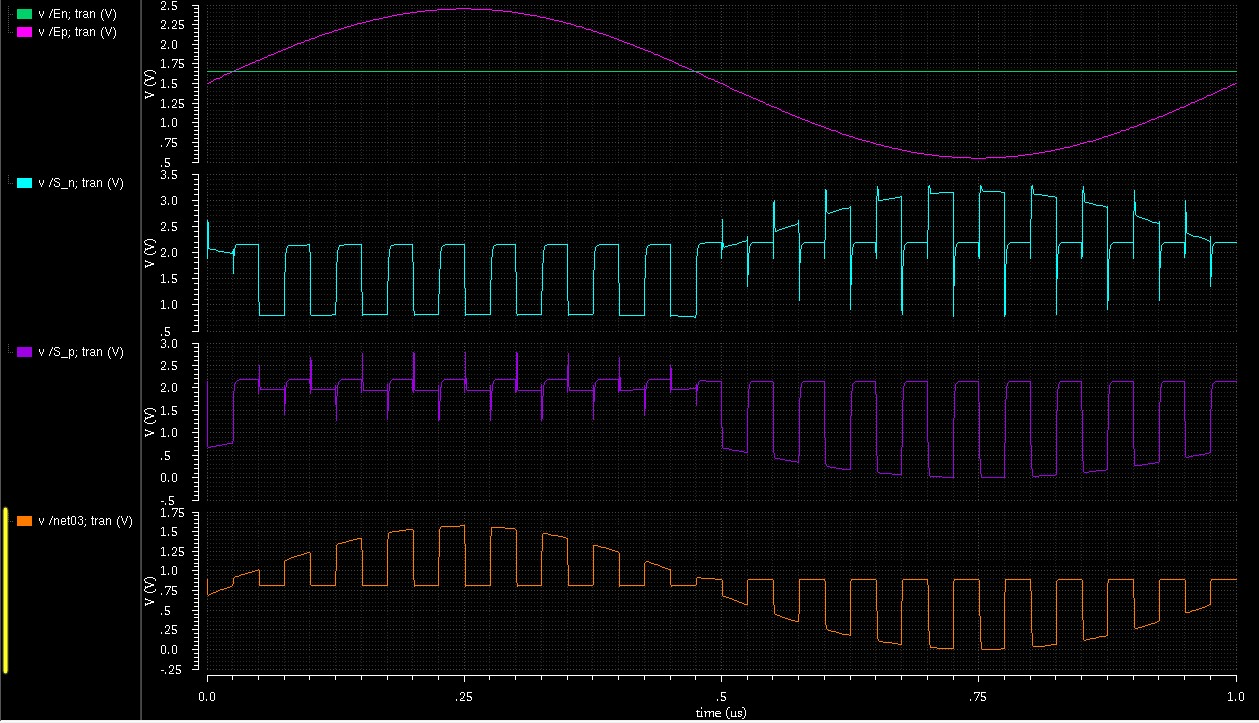
\includegraphics[width=0.8\linewidth]{sim_comp_before_SR_FF.jpg}
      \caption{Simulation avant l'ajout des buffers + bascules}
      \label{fig:sfigBSRFF}
\end{figure}%

Nous avons donc rajout\'e des inverseurs et une Bascule SR (en 2 Nandes interconnect\'ees) en sortie afin de m\'emoriser
un 0 ou un 1 logique.

\begin{figure}[!htb]
      \centering
      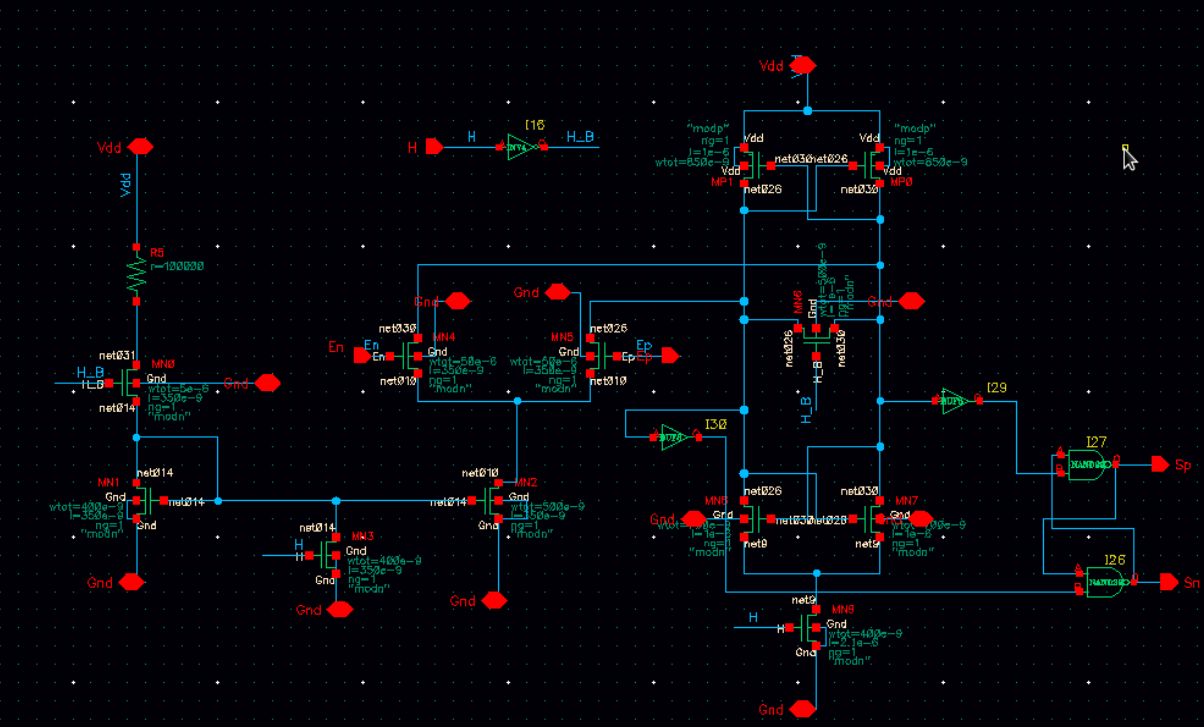
\includegraphics[width=0.9\linewidth]{comparateur_schema_cadence_SR.png}
      \caption{Sch\'ema \'electrique}
      \label{fig:schcompSR}
\end{figure}%

\begin{figure}[!htb]
      \centering
      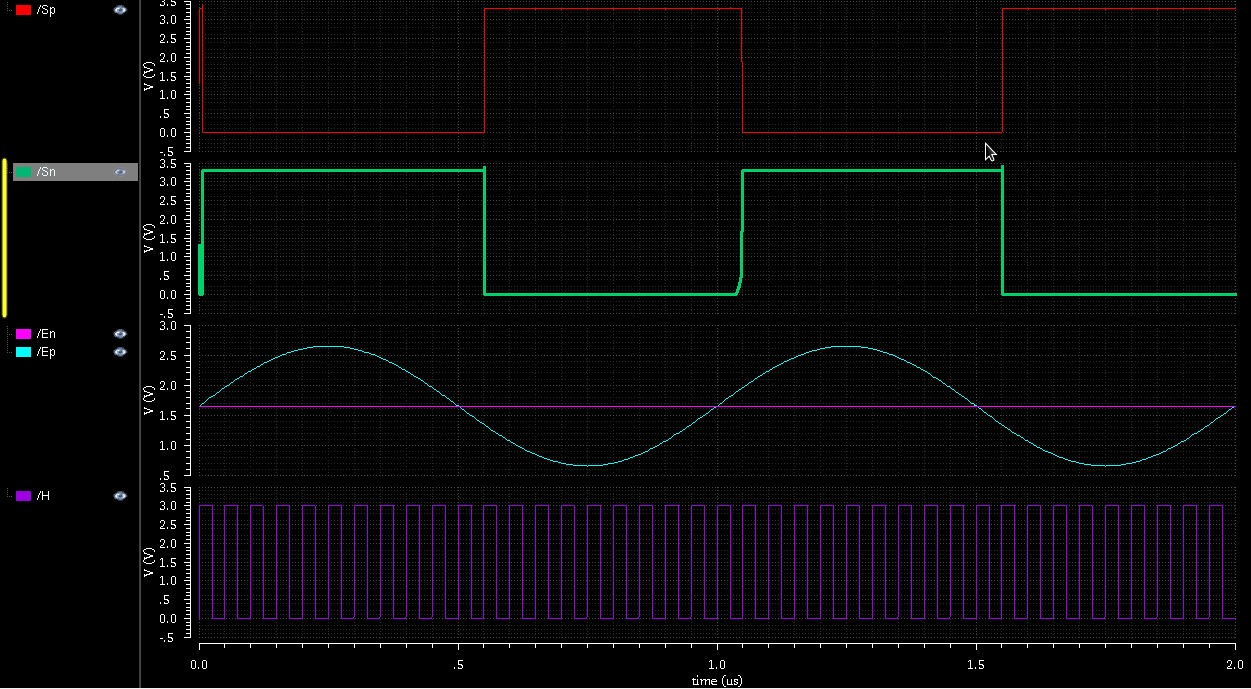
\includegraphics[width=\linewidth]{sim_comp_after_SR_FF.jpg}
      \caption{Simulation apr\`es l'ins\'ertion de ces \'el\'ements}
      \label{fig:sfigASRFF}
\end{figure}%


\iffalse
\begin{figure}[!htb]
  \begin{subfigure}{.5\textwidth}
      \centering
      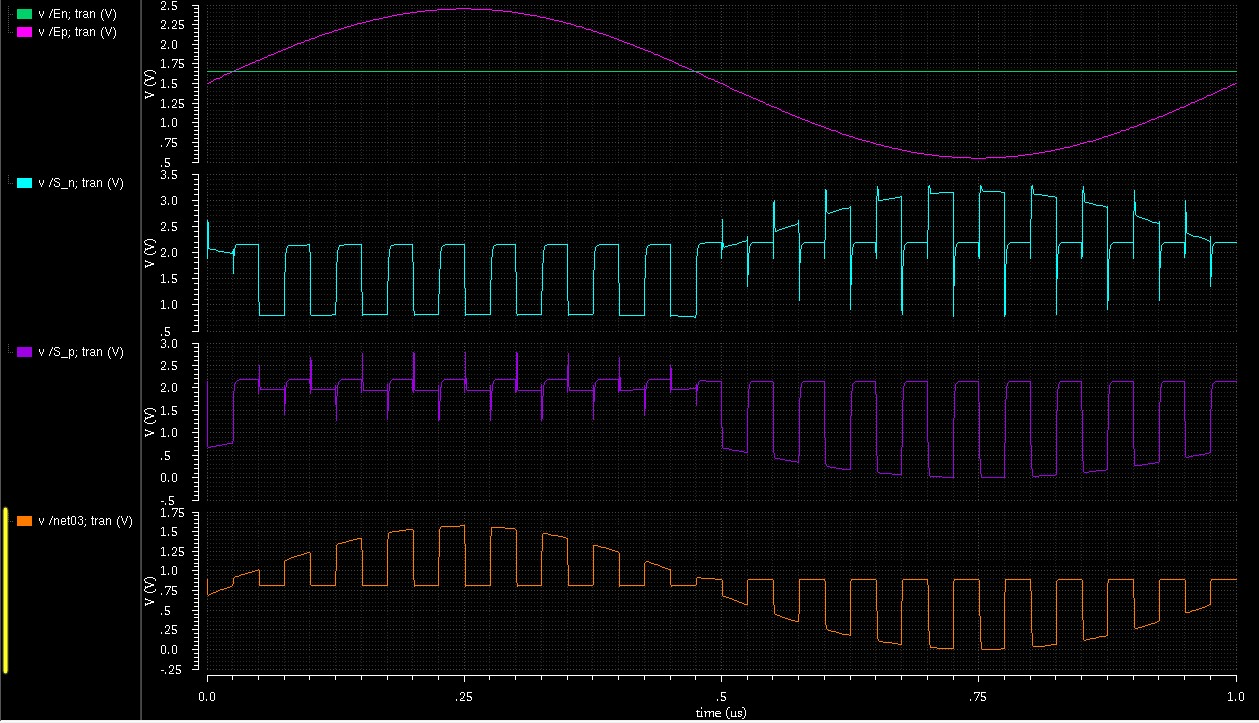
\includegraphics[width=1.2\linewidth]{sim_comp_before_SR_FF.jpg}
      \caption{Simulation avant l'ajout des buffers + bascules}
      \label{fig:sfigBSRFF}
  \end{subfigure}%

  \begin{subfigure}{.5\textwidth}
    \centering
    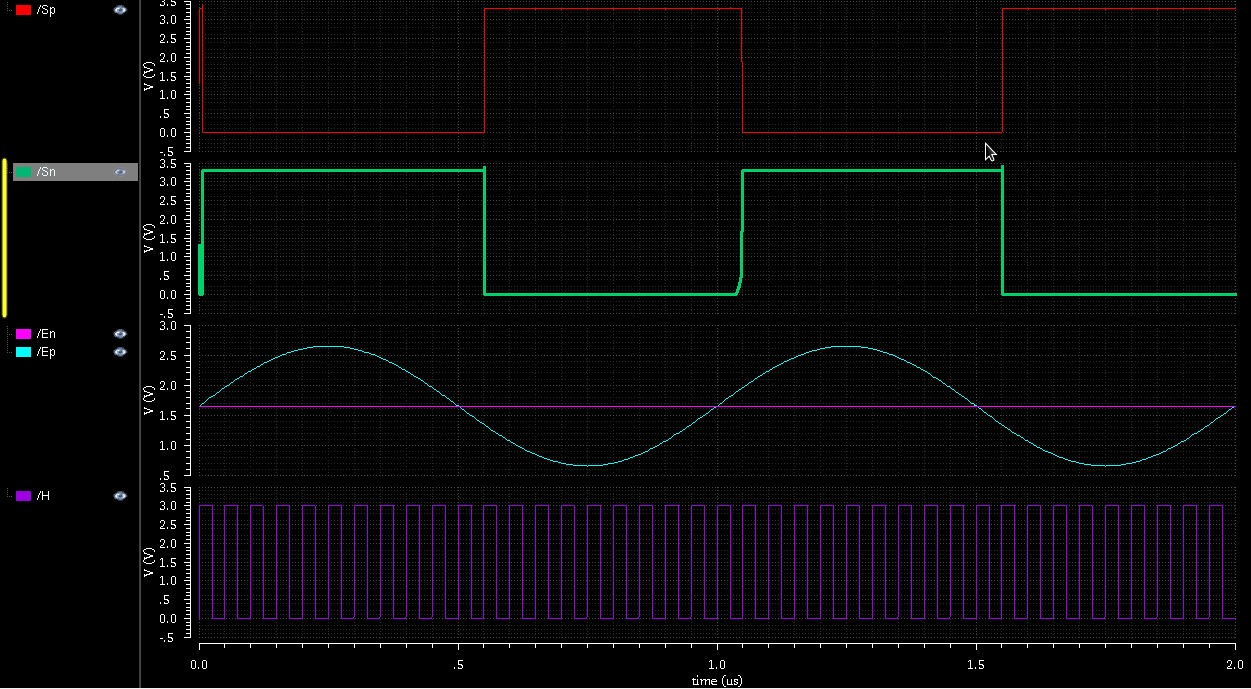
\includegraphics[width=1.2\linewidth]{sim_comp_after_SR_FF.jpg}
    \caption{Simulation apr\`es l'ins\'ertion de ces \'el\'ements}
    \label{fig:sfigASRFF}
  \end{subfigure}

  \caption{Diff\'erence en sortie en simulation entre comparateurs sans/avec bascule SR respectivement}
  \label{fig:figcomp}
\end{figure}
\fi

\iffalse
\subsubsection{Imp\'edance diff\'erentielle n\'egative et expression du Gain}
\subsubsection{D\'etermination du courant et dimensionnements}
\fi

\clearpage

\section{R\'ealisation du d\'ecodeur en Verilog}
\subsection{Programmation et synth\`ese automatique du circuit}
On utilise un code existant en Verilog\cite{Thermometer}
Ce code permet de convertir les donn\'ees en code thermometrique en sortie des
comparateurs vers un code binaire sur 6 bits (avec un pouvoir de bulles).

\begin{lstlisting}[language=Verilog, belowskip=-0.5 \baselineskip]
module thermo2bin (thermob, bin)
input[62:0] thermob;
output [5:0] bin;

reg [62:0] thermo;
reg [5:0] bin, bin1, bin2;
integer i, j, k;

always @(thermob)
begin
  for (k = 0; k <=60; k=k+1)
    thermo[k] <= thermob[k] || thermob[k+1] || thermob[k+2];

  thermo[61] <= thermob[61] || thermob[62];
  thermo[62] <= thermob[62];
end

always @(thermo)
begin
  bin1 = 0;
  for(i=1; i <= 32; i=i+1)
    if (thermo[i-1] = 1'b1) bin1 = i;
end

always @(thermo)
begin
  bin2 = 0;
  for(j=1; j<=31; j=j+1)
    if(thermo[k+31] == 1'b1) bin2 = j;
end

always @(bin1 or bin2)
if (thermo[31] == 1'b1)
  bin = bin2 + 32;
else
  bin = bin1;

endmodule

\end{lstlisting}

\subsubsection{Fonctionnement}

Ce module fonctionne du m\^eme principe de la lecture humaine : On essaye de lire le plus
haut '1'. Ce bout de code \'etait optimis\'e pour qu'il fonctionne en 2 parties

\textbf{\textcolor{red}{+explications..\cite{Thermometer}}}

\subsubsection{Synth\`ese}

\clearpage
\subsection{Simulations}

\begin{figure}[!htb]
      \centering
      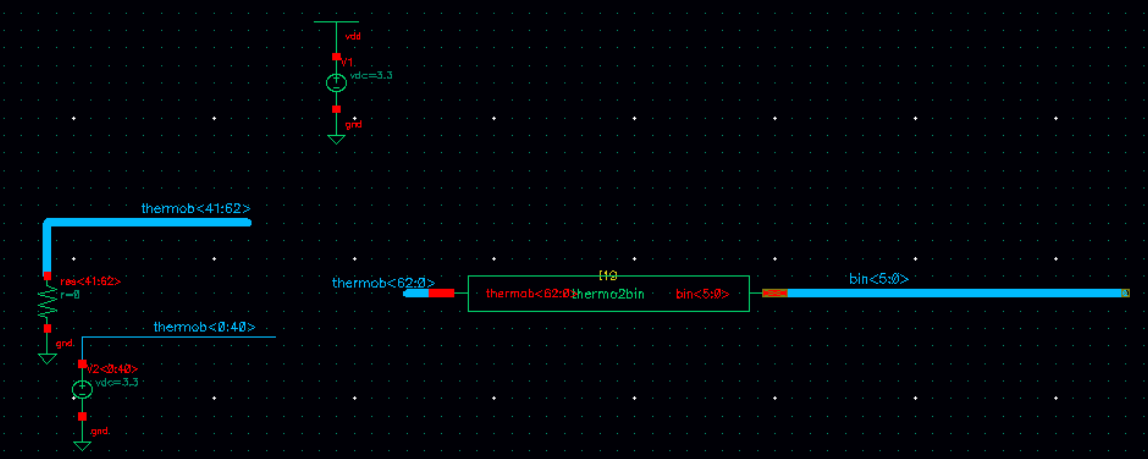
\includegraphics[width=\linewidth]{test_thermo2bin.png}
      \caption{Placement d'un band de test pour le code Verilog apr\`es synth\`ese.}
\end{figure}%

\clearpage


\section{Sch\'ema Global}
\subsection{Mise en place des \'el\'ements du montage final}
La mise en oeuvre du sch\'ema final se fait par le placement de l'\'echantillonneur bloqueur
ainsi que les 63 comparateurs et le pont de r\'esistance pour la cr\'eation des seuils.

En soi, le sch\'ema est celui de la figure X :

\iffalse
\begin{center}
\textbf{\textcolor{red}{Sch\'ema du l'\'echantillonneur-Bloqueur + CAN-FLASH \`a faire}}.\\
\end{center}
\fi

\begin{figure}[!htb]
\begin{center}
  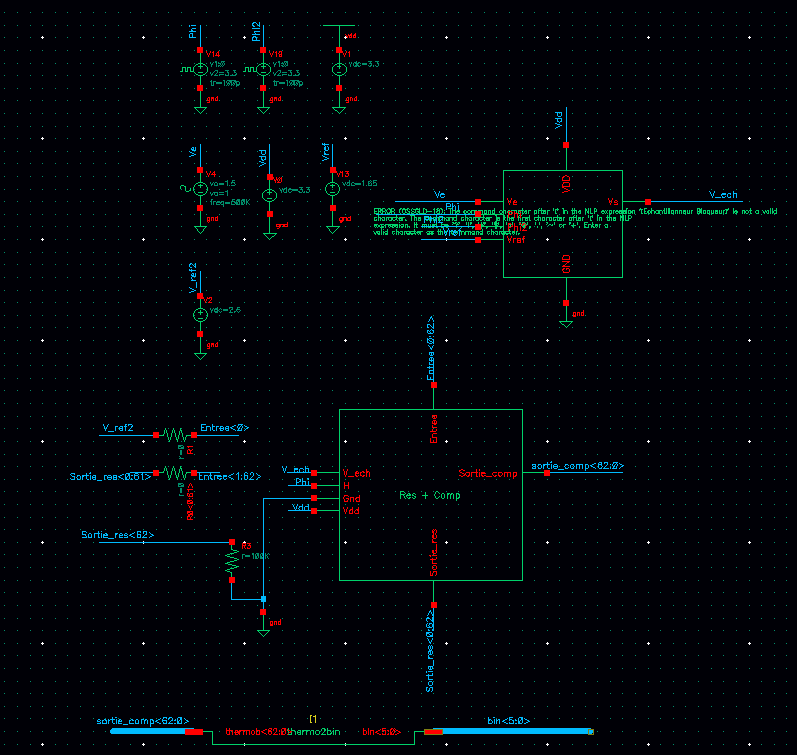
\includegraphics[scale=0.50]{schema_final.png}
  \caption{"Sch\'ema global du CAN-FLASH"}
\end{center}
\end{figure}

Lors de cette \'etape, nous avons utilis\'e un bloc ``Comparateur + r\'esistance'' que nous avons boucl\'e
sur lui-m\^eme 62 fois dans le but d'\'eviter le sch\'ema \`a rallonge (avec 63 bo\^ites diff\'erentes…).
L'entr\'ee du premier bloc de comparaison (comparateur et seuil gr\^ace \`a la r\'esistance) prend en compte
le signal en sortie de l'\'echantillonneur bloqueur ainsi que le niveau de r\'ef\'erence le plus haut.
Le second \'etage de comparaison a pour entr\'ee la sortie de premier \'etage ainsi que le signal \'echantillonn\'e.
Cet \'etage compare donc le signal \'echantillonn\'e et le seuil num\'ero 2 (deux r\'esistances \'egales en s\'erie).

Le dernier \'etage de comparaison utilise toujours le m\^eme signal \'echantillonn\'e ainsi que le seuil 64 form\'e
de 64 r\'esistances en s\'erie.

\subsection{Simulations}

La simulation globale de cet \'etage est tr\`es int\'eressante. En effet, les courbes pr\'esentent des valeurs de
seuils tr\`es diff\'erentes de celles \textcolor{red}{pressenties} par le calcul (niveaux nets cr\'es par des r\'esistances en s\'erie).
En fait, les entr\'ees des comparateurs sont des gros transistors NMOS. Par cons\'equent, leurs capacit\'es d'entr\'ee
sont tr\`es importantes ; une fois reli\'ees \`a des r\'esistances (pont de r\'esistances), des effets de filtrages
apparaissent et d\'egradent les niveaux de seuils.

Les filtres ont en moyenne une fr\'equence de coupure de $\frac{1}{2 \pi R C}$ avec $C  = 90 \phantom{2} fF.$
Pour pallier ce ph\'enom\`ene, nous avons plac\'e un suiveur parfait (vcvs) dans la bo\^ite de comparaison pour
`` purifier '' les niveaux de seuils.

\subsection{Etage de d\'ecodage}

Mettre une bascule \`a la fin du comparateur pour bien synchro avec le d\'ecodeur.

\clearpage

\section{Layout}
\subsection{Mise en oeuvre}

\begin{figure}[!htb]
      \centering
      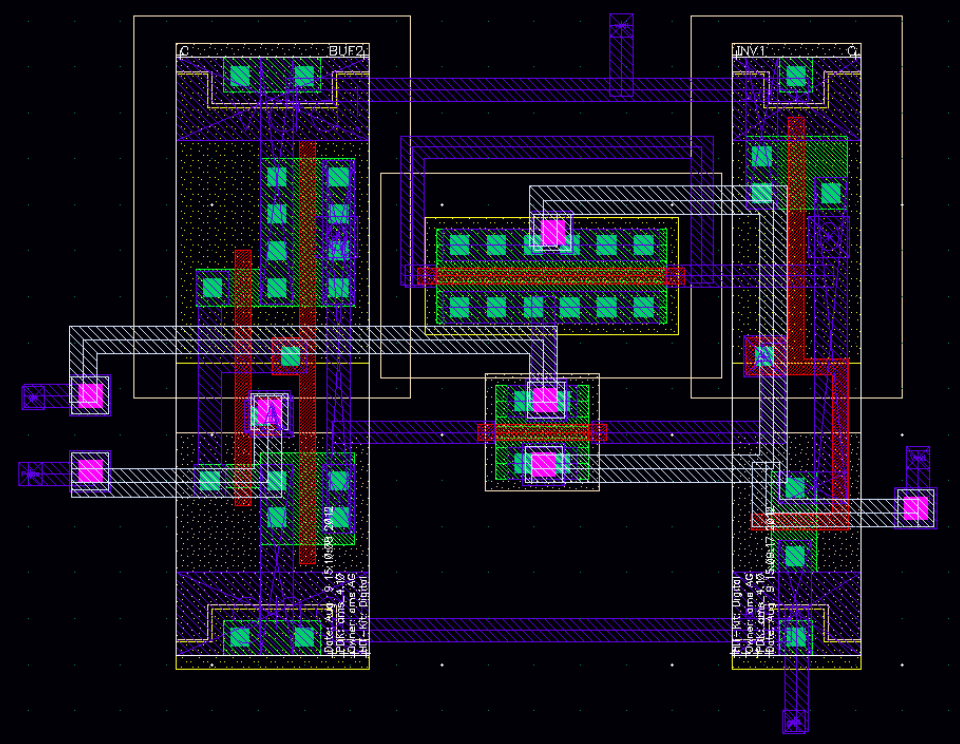
\includegraphics[width=0.6\linewidth]{layout_.png}
      \caption{Mise en place du layout d'un switch}
\end{figure}%

\clearpage

\section{Am\'eliorations possibles}

Finalement, notre convertisseur fonctionne presque parfaitement : l'\'etage d'\'echantillonneur bloqueur remplit tout \`a fait son r\^ole.
En revanche, certains \'etages de comparaison n'affichent pas toujours la bonne valeur. Th\'eoriquement, si l'\'etage de comparaison n sort
la valeur 1 en code thermom\'etrique, les \'etages $>$ n doivent \'egalement afficher 1 et $<$ n, 0 Dans nos simulations, il arrive que des \'etages
sup\'erieurs soient \`a 0.

Nous soup\c connons les inverseurs et portes NAND de mal interpr\'eter la tension en sortie d'un comparateur et de mal traduire l'information.
Pour contrer ces probl\`emes mineurs (moins d'une comparaison fausse sur 10), il faudrait revoir la partie droite de l'\'etage de comparaison
concernant le latch et la polarisation de sortie. On pourrait par exemple optimiser la puissances des portes logiques ou calculer avec de
plus fins mod\`eles les caract\'eristiques des transistors concern\'e sur le comparateur.

L'\'etage d\'ecodeur de code thermom\'etrique vers binaire fonctionne parfaitement mais est impact\'e par le probl\`eme susmentionn\'e de fausse comparaison.
Il en r\'esulte une erreur d'environ trois valeurs sur 64 ce qui fausse le code binaire final.

\section{Conclusion}

La r\'ealisation d'un CAN Flash 6 bits pr\'esent\'ee dans ce projet fut une bonne exp\'erience dans la mesure o\`u nous sommes d\'esormais conscients
de la complexit\'e \`a r\'ealiser un convertisseur efficace et s\^ur.
Le d\'ebut du projet fut d\'elicat car nous \'etions confront\'es \`a de lourds sch\'emas \'electriques \`a r\'ealiser. Leur optimisation prit du temps et
passa par de nombreux calculs th\'eoriques vus en cours de convertisseurs ou d'\'electronique analogique.
Ce projet fut \'egalement l'occasion de v\'eritablement prendre en main le logiciel Virtuoso de Cadence \`a travers les outils de simulation,
 de variables ajust\'ees, de sources de courant ou tension parfaites. Nous maîtrisons d\'esormais ce logiciel et sommes aptes \`a l'utiliser \`a
 des fins de recherche ou dans l'industrie.

Nous sommes ravis d'avoir pu r\'efl\'echir par nous-même et mobiliser nos connaissances acquises dans plusieurs cours cette ann\'ee au service
de ce projet. Il a eu un r\'eel impact sur notre maîtrise de Cadence et sur le d\'eroulement de la phase de conception d'un circuit \'electronique,
en l'occurrence d'un comparateur Flash.

Nous remercions les professeurs encadrants de nous avoir transmis leurs connaissances et astuces dans le domaine, nous les utiliserons
\`a bon escients \`a l'avenir.

\clearpage

\section{Fiche descriptive des caract\'eristiques}

\clearpage

\section{Annexes}

\clearpage

\addcontentsline{toc}{section}{R\'ef\'erences}

\begin{thebibliography}{9}
\bibitem{Razavi}
\textit{Design of Analog CMOS Integrated Circuits}
\\\texttt{Behzad Razavi, McGraw-Hill Higher Education.}

\bibitem{Razavi Data-Conversion}
\textit{AnalogtoDigital Converter Architectures}
\textit{in Principles of Data Conversion System Design}\\
\texttt{Behzad Razavi, Wiley-IEEE Press, 1995, pp.96-152}.\\
\textbf{doi: 10.1109/9780470545638.ch6}

\bibitem{Thermometer}
\textit{Verilog HDL model based thermometer-to-binary encoder with bubble error correction}\\
\texttt{Zbigniew Jaworski, Warsaw University of Technology}\\
\textit{Conference: 2016 MIXDES - 23rd International Conference "Mixed Design of Integrated Circuits and Systems"}\\
\textbf{doi: 10.1109/MIXDES.2016.7529741}

\end{thebibliography}


\end{document}
